\begin{figure*}
\centering
\begin{subfigure}[b]{0.32\textwidth}
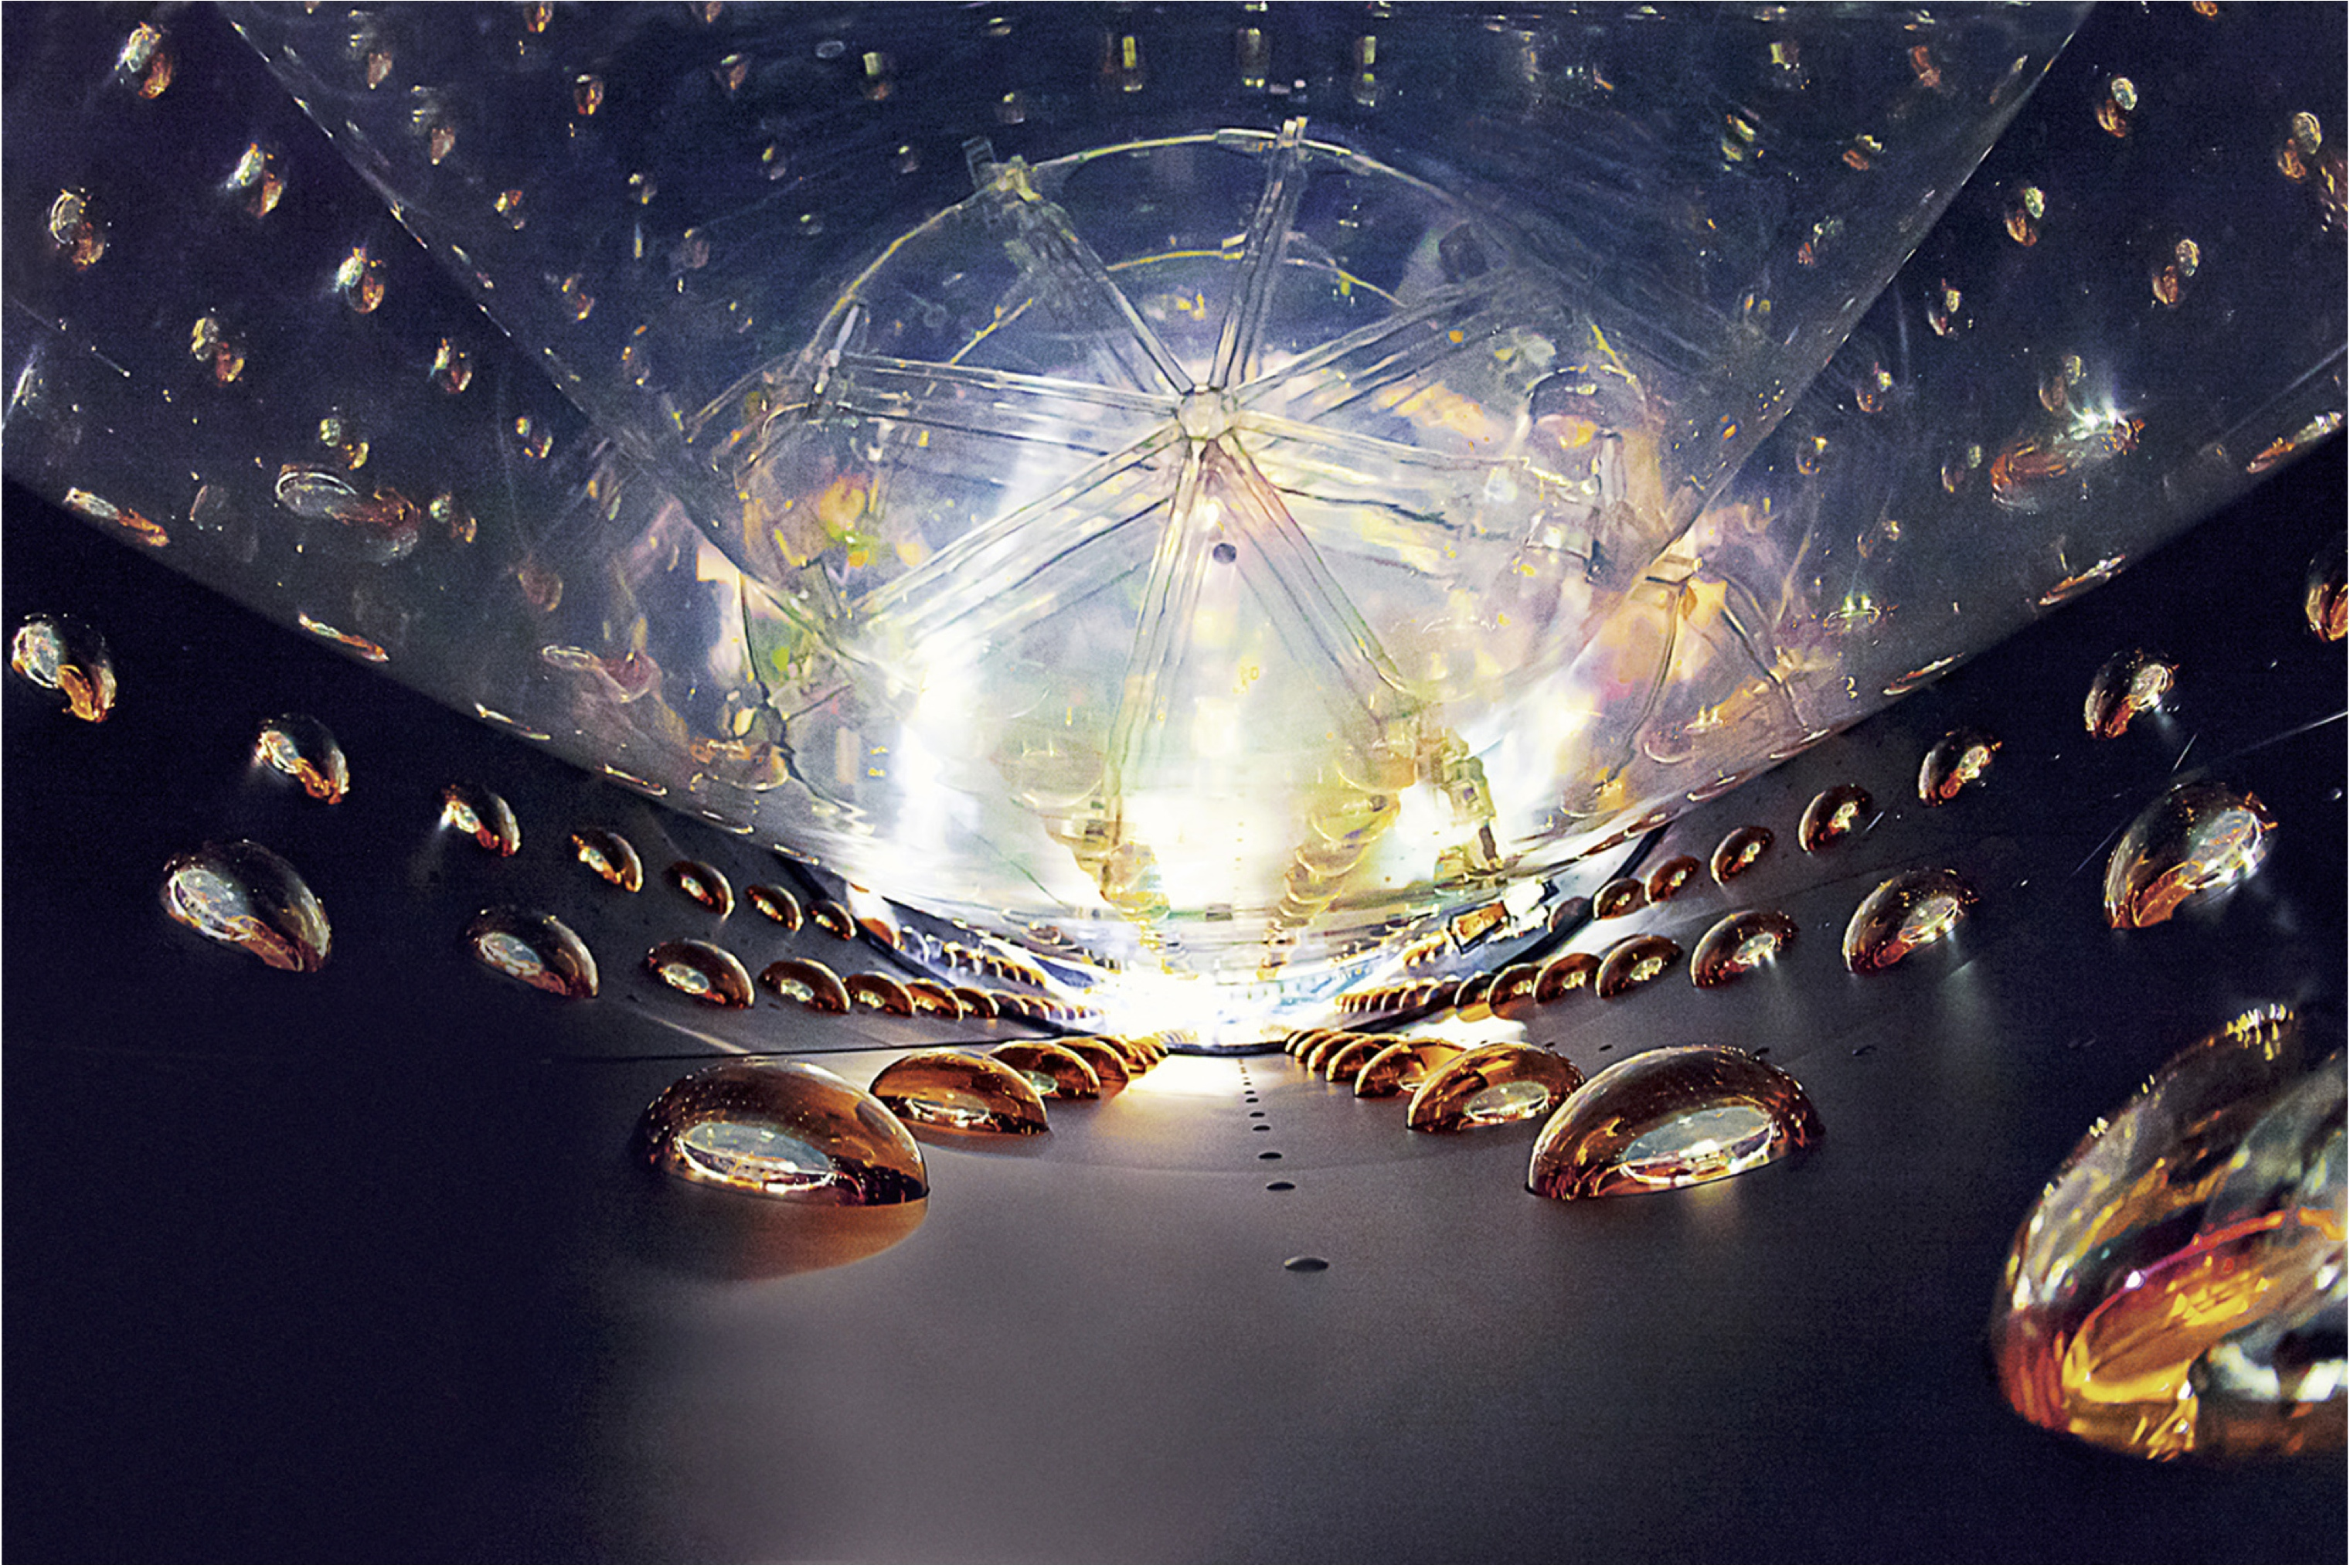
\includegraphics[width=\textwidth]{fig/dayabay.jpg}
\caption{Daya Bay Neutrino Experiment}
\label{fig:dayabay}
\end{subfigure}
\begin{subfigure}[b]{0.42\textwidth}
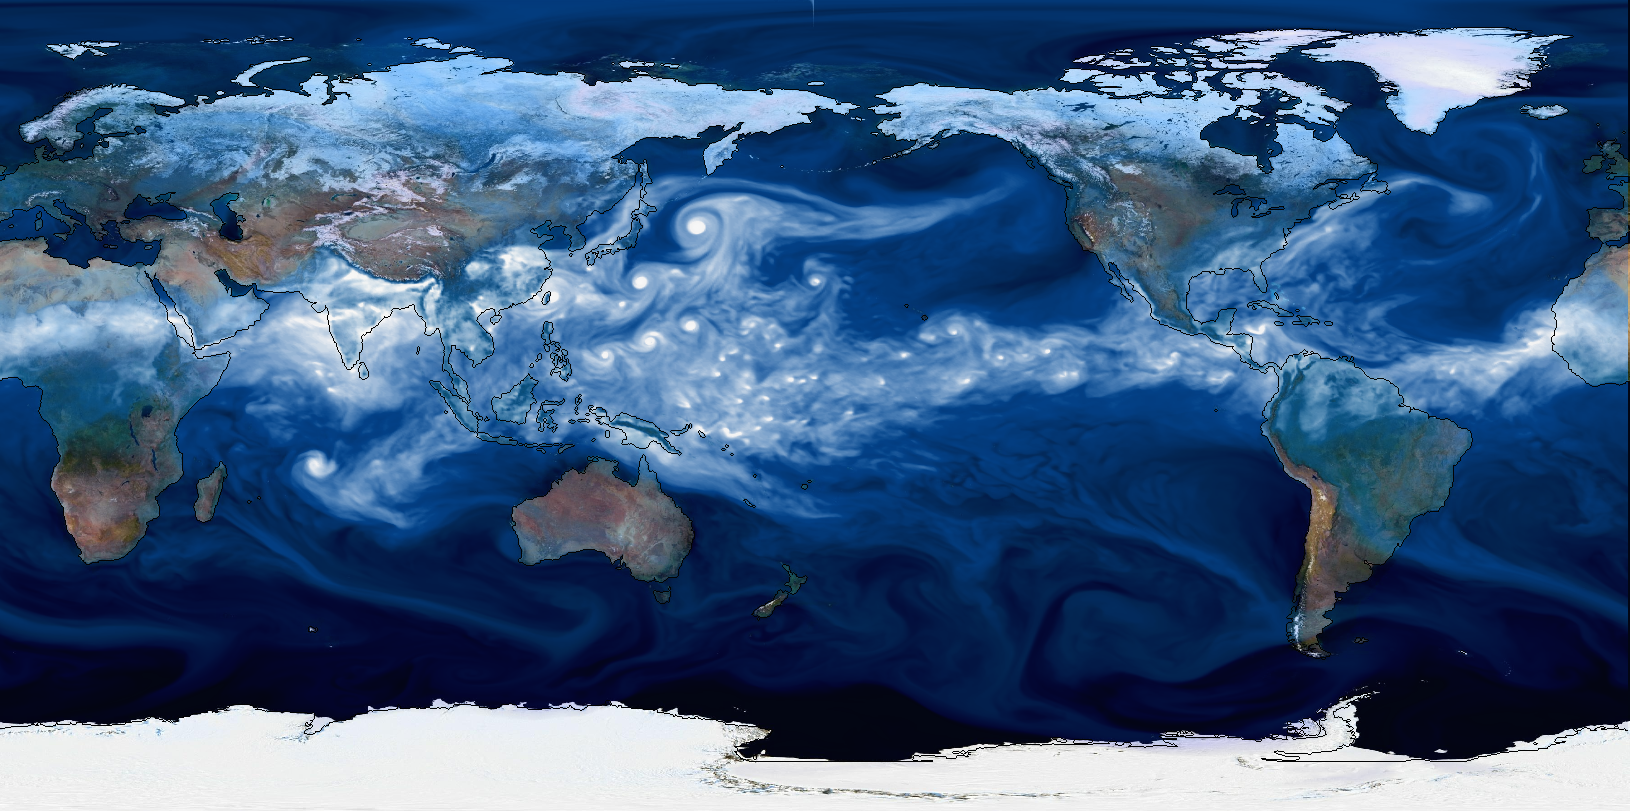
\includegraphics[width=\textwidth]{fig/climate.png}
\caption{CAM5 Simulation}
\label{fig:cam5}
\end{subfigure}
\begin{subfigure}[b]{0.22\textwidth}
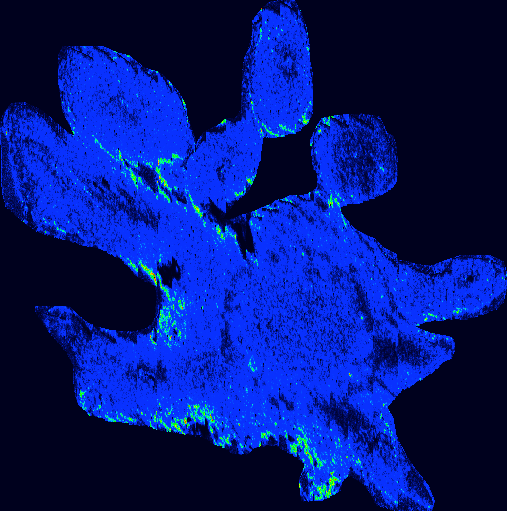
\includegraphics[width=\textwidth]{fig/mass-spec.png}
\caption{Mass-Spec Imaging}
\label{fig:mass-spec}
\end{subfigure}
\caption{Sources of various datasets used in this study}\label{fig:datasets}
\end{figure*}
In this study, we choose leading datasets from experimental, observational, and simulation sources, and we identify associated data analytics challenges. 
%We compare the performances of our MPI and Spark implementations of the low-rank decompositions on: a 1.6TB-sized sparse matrix obtained from the Daya Bay Neutrino Experiment for NMF decomposition;  a 2.2TB and 16TB-sized dense matrix of oceanic (reanalysis) and atmospheric (simulation) variables for PCA decomposition; and a 1TB-sized sparse matrix obtained via mass spectrometry imaging for  CX decomposition. All matrices were processed in double precision. 
The properties of these datasets are summarized in Table~\ref{table:datasets}.

\begin{table}[ht]
\centering
\caption{Summary of the matrices used in our study}
\label{table:datasets}
\begin{tabular}{p{2cm}lllll@{}}
\toprule
Science Area & Format/Files & Dimensions & Size  \\ \midrule
MSI      & Parquet/2880        &  $8,258,911 \times 131,048$          & 1.1TB  \\
Daya Bay & HDF5/1      &   $1,099,413,914 \times 192$         & 1.6TB \\
Ocean              & HDF5/1      &  $6,349,676 \times 46,715$          & 2.2TB \\
Atmosphere           & HDF5/1       & $26,542,080 \times 81,600$           & 16TB \\ \bottomrule
\end{tabular}
\end{table}



\paragraph{The Daya Bay Neutrino Experiment.}
The Daya Bay Neutrino Experiment (Figure \ref{fig:dayabay}) is situated on the southern coast of China. It detects antineutrinos produced by the Ling Ao and Daya Bay nuclear power plants and uses them to measure theta-13, a fundamental constant that helps describe the flavor oscillation of neutrinos. In 2012 the Daya Bay experiment measured this with unprecedented precision. This result was named one of the Science magazines top ten breakthroughs of 2012, and this measurement has since been refined considerably \cite{dayabay15}.

The Daya Bay Experiment consists of eight smaller detectors, each with 192 photomultiplier tubes that detect light generated by interaction of anti-neutrinos from the nearby nuclear reactors. Each detector records the total charge in each of the 192 photomultiplier tubes, as well as the time the charge was detected. For this analysis we used a data array comprised of the sum of the charge for every photomultiplier tube from each Daya Bay detector. This data is well suited to NMF analysis since accumulated charge will always be positive (with the exception of a few mis-calibrated values). The extracted data was stored as HDF5 files with 192 columns, one for each photomultiplier tube, and a different row for each discrete event in the detectors. The resulting dataset is a sparse 1.6 TB matrix. The specific analytics problem that we tackle in this paper is that of finding characteristic patterns or signatures corresponding to various event types. Successfully ``segmenting'' and classifying a multiyear long timeseries into meaningful events can dramatically improve the productivity of scientists and enable them to focus on anomalies, which can in turn result in new physics results.

\paragraph{Climate Science.}
Climate change is one of the most pressing challenges facing human society in the 21st century. Climate scientists rely on HPC simulations to understand past, present and future climate regimes. Vast amounts of 3D data (corresponding to atmospheric and ocean processes) are readily available in the community. Traditionally, the lack of scalable analytics methods and tools has prevented the community from analyzing full 3D fields; typical analysis is thus performed only on 2D spatial averages or slices. 

In this study, we consider the Climate Forecast System Reanalysis Product~\cite{saha:2010}. Global Ocean temperature data, spatially resolved at 360 x 720 x 41 (latitude x longitude x depth) and 6-hour temporal resolution is analyzed. The CFSR dataset yields a dense 2.2TB matrix. We also process a CAM5 0.25-degree atmospheric humidity dataset~\cite{wehner:2014} (Figure  \ref{fig:cam5}). The grid is 768 x 1158 x 30 (latitude x longitude x height) and data is stored every 3 hours. The CAM5 dataset spans 28 years, and it yields a dense 16TB matrix. The specific analytics problem that we tackle is finding the principal causes of variability in large scale 3D fields. PCA analysis is widely accepted in the community; however the lack of scalable implementations has limited the applicability of such methods to TB-sized datasets.  
%We apply our PCA implementations to the analysis of ocean temperatures collected in 6 hours increments over a global  latitude-longitude-depth grid, extracted from the . Unfolding each 3D grid set of temperature measurements into a long vector and taking the vectors formed in this way to be columns of a matrix yields a dense 2.2TB matrix. Further, we also compute the EOFs of 28 years of measurements of atmospheric variable collected at 3 hours increments over a global 768-by-1152-by-30 latitude-longitude-height grid, \textcolor{red}{what is the provenance?}. Forming the matrix as in the case of the ocean temperatures yields a dense 16TB matrix. To the best of our knowledge, this is the first published work where climate fields of these sizes have been subjected to EOF analysis.
%The most widely used tool for extracting important patterns from the measurements of atmospheric and oceanic variables is the Empirical Orthogonal Function (EOF) technique. EOFs are popular because of their simplicity and their ability to reduce the dimensionality of large nonlinear, high-dimensional systems into fewer dimensions while preserving the most important patterns of variations in the measurements. Mathematically, EOFs are exactly PCA decompositions.
%Traditionally, EOFs have been calculated on two-dimensional slices of fields due to the difficulties climate scientists face when attempting to apply their usual computational tools to the immense amount of data present in the full 3D fields.· %The EOF modes extracted in this manner project the true complex 3D patterns involving multiple layers of the atmospher or ocean onto the considered slice. A better understanding of the dynamics of large-scale modes of variability in the ocean and atmosphere may be extracted from full 3D EOFs.
\paragraph{Mass-Spectrometry Imaging.}
Mass spectrometry measures ions derived from the molecules present in a biological sample. Spectra of the ions are acquired at each location (pixel) of a sample, allowing for the collection of spatially resolved mass spectra. This mode of analysis is known as \textit{mass spectrometry imaging (MSI)}. The addition of \textit{ion-mobility separation (IMS)} to MSI adds another dimension, drift time.  The combination of IMS with MSI is finding increasing applications in the study of disease diagnostics, plant engineering, and microbial interactions. Unfortunately, the scale of MSI data and complexity of analysis presents a significant challenge to scientists: a single 2D-image may be many gigabytes and comparison of multiple images is beyond the processing capabilities available to many scientists. The addition of IMS exacerbates these problems. 

We analyze one of the largest (1TB sized) mass-spec imaging datasets in the field, obtained from a sample of the plant {\it Lewis Dalisay Peltatum} (Figure \ref{fig:mass-spec}). The MSI measurements are formed into a sparse matrix whose rows and columns correspond to pixel and ($\tau$, $m/z$) values of ions, respectively. Here $\tau$ denotes drift time and $m/z$ is the mass-to-charge ratio. The sheer size of this dataset has previously made complex analytics intractable. CX decompositions allow for the possibility of identifying small numbers of columns (ions) in the original data that reliably explain a large portion of the variation in the data.


